\section{Rectangular targets and the corner cube}\label{sec:corner}
The simplest target is rectangular: $\Lambda'=\bigoplus_io_i\Z$, which has Graver set $\{\pm o_ie_i\}$. This includes $\Lambda'=\Z^k$ (all $o_i=1$), the case $b'=1$. For rectangular targets the realised union has an explicit complement and the transport question becomes exact.

\subsection{Gap reduction}
\begin{lemma}[coverage-gap reduction]\label{lem:gap}
Let $F\subseteq F'$ and let $H=\conv F\subseteq H'=\conv F'$. Put $\mathcal G'=H'\setminus U'$. Then $U\setminus U'=U\cap\mathcal G'$. Hence $U\subseteq U'\iff U\cap\mathcal G'=\emptyset$, and $U'=H'$ implies $U\subseteq U'$.
\end{lemma}
\prov{CW-0476}{P3-T0}{PROVED}{FULL}
\begin{proof}
Every cell is the convex hull of its vertices, so $U\subseteq H\subseteq H'$. A point of $U$ outside $U'$ therefore lies in $H'\setminus U'$, and conversely. \qedhere
\end{proof}

\subsection{The corner-cube criterion}
Fix a rectangular target $\Lambda'=\bigoplus o_i\Z$, a source $\Lambda$ with $F(\Lambda,Q)\subseteq F(\Lambda',Q)$, and assume $\tilde Q_i=\lfloor q_i/o_i\rfloor\ge1$ for all $i$ (if some $\tilde Q_i=0$, the coordinate carries no point of $F'\supseteq F$ and the problem is the same problem in $k-1$ coordinates). Put $A_i=o_i\tilde Q_i$, $B=\prod[0,A_i]$ and let $O=\{z\in\R^k:z_i<o_i\ \forall i\}$ be the \emph{open corner cube}.
\begin{theorem}[corner-cube criterion]\label{thm:corner}
(a) $U'=B\setminus O=\{z\in B:\max_iz_i/o_i\ge1\}$.
(b) $U\subseteq U'\iff U\cap O=\emptyset\iff$ no cell of $\Kabs(\Lambda,Q)$ meets $O$.
(c) If $U\cap O\ne\emptyset$, the scaled lattice $\tilde\Lambda=\mathrm{diag}(o)^{-1}\Lambda$ contains a nonzero vector $v\ge0$ with $|v|_1\le k-1$.
(d) No cell of dimension $\le1$ meets $O$, in any dimension $k$.
(e) If $k=2$ then $U\subseteq U'$ (for every rectangular target, including $\Z^2$).
(f) If a $k$-cell meets $O$, then one of its $(k-1)$-faces (itself a cell) meets $O$. Hence for $k=3$ every obstruction is carried by a $2$-cell.
\end{theorem}
\prov{CW-0479}{P3-T3}{PROVED}{FULL}
\begin{proof}
(a) The Graver vectors of $\Lambda'$ in $[-q,q]$ are $\pm o_ie_i$, so the cells of $\Kabs(\Lambda',Q)$ are the faces $\prod I_i$ of the grid cubes $\prod[n_io_i,(n_i+1)o_i]$ ($0\le n_i<\tilde Q_i$), with $I_i$ either an endpoint or the interval, all of whose corners are nonzero. ($\supseteq$) Let $z\in B$ with $z_{i_0}\ge o_{i_0}$ for some $i_0$. Put $I_i=\{z_i\}$ if $z_i/o_i\in\Z$ and $I_i=[n_io_i,(n_i+1)o_i]$ with $n_i=\lfloor z_i/o_i\rfloor$ otherwise (then $z_i<A_i$, so $(n_i+1)o_i\le A_i$). Then $\Phi=\prod I_i$ is a grid face containing $z$ whose every vertex has $i_0$-th coordinate $\ge o_{i_0}>0$ (if $I_{i_0}$ is an interval then $n_{i_0}\ge1$; otherwise $I_{i_0}=\{z_{i_0}\}$); so $0$ is not a vertex of $\Phi$, $\Phi$ is a cell, and $z\in U'$. ($\subseteq$) A cell is a grid face $\prod I_i$ that does not have $0$ as a vertex; $0$ is a vertex iff every $I_i$ has lower endpoint $0$, so some $I_i\subseteq[o_i,\infty)$ and every point of the cell has $z_i\ge o_i$.

(b) $U\subseteq H\subseteq\conv F'\subseteq B$, so $z\in U\setminus U'$ iff $z\in U\cap O$ by (a).

(c) Let $z\in U\cap O$ lie in a cell with vertices $v^{(j)}\in F\subseteq\Lambda$ and $z=\sum\lambda_jv^{(j)}$ (convex). In scaled coordinates $\tilde v^{(j)}\in\N^k\setminus\{0\}$ and $\sum_i\tilde z_i<k$ because each $\tilde z_i<1$, while $\sum_i\tilde z_i=\sum_j\lambda_j|\tilde v^{(j)}|_1$. So some vertex has $|\tilde v|_1<k$.

(d) A $0$-cell is a nonzero point of $\N^k$ in scaled coordinates, hence has a coordinate $\ge1$ and is not in $O$. Let $[P,R]$ be an edge, $P,R\in F$, $g=R-P\in\Gr(\Lambda)$ (either orientation), and suppose $z=(1-t)P+tR\in O$. In scaled coordinates $\tilde z_i<1$ forces $\tilde P_i=0$ or $\tilde R_i=0$ for each $i$ (if both were $\ge1$, then $\tilde z_i\ge1$): the supports are disjoint. Then $\tilde g=\tilde R-\tilde P$ agrees with $\tilde R$ on $\supp\tilde R$ and is $\le0$ where $\tilde P\ne0$, so $R\cm g$, $R\in\Lambda\setminus\{0\}$, and $R\ne g$ because $P\ne0$. Thus $g$ is not conformally minimal, a contradiction.

(e),(f) Let $C$ be a $k$-cell with $C\cap O\ne\emptyset$ and suppose $\partial C\cap O=\emptyset$. The cube $O$ is connected and $O=(O\cap\mathrm{int}\,C)\sqcup(O\setminus C)$ with both parts open, the first nonempty; so $O\subseteq\mathrm{int}\,C$ and $0\in\overline O\subseteq C$. All vertices of $C$ lie in the closed orthant, hence so does $C$; $0$ is an extreme point of the orthant, so $0$ is an extreme point of $C$, i.e.\ a vertex, but vertices lie in $F\not\ni0$. This contradiction shows $\partial C\cap O\ne\emptyset$; $\partial C$ is the union of the $(k-1)$-faces, which are cells. For $k=2$ these faces are edges, which miss $O$ by (d); cells of dimension $\le1$ miss $O$ by (d); so $U\cap O=\emptyset$ and (b) gives $U\subseteq U'$. \qedhere
\end{proof}
\begin{remark}[why dimension two is special]\label{rem:dim}
By (c) a failure needs a nonzero vertex of $\ell_1$-size at most $k-1$ in scaled coordinates. For $k=2$ this means a scaled vertex $e_i$, a configuration already excluded by (d)--(e); for $k=3$ the size $2$ is reached by vectors such as $(1,1,0)$, which exist in the even-sum lattice, and by (f) the cells that obstruct are squares. This is the first place where dimension enters; the planar hard-cell mechanism of \cref{sec:planar} is its non-rectangular analogue.
\end{remark}
\begin{figure}[tbp]\centering
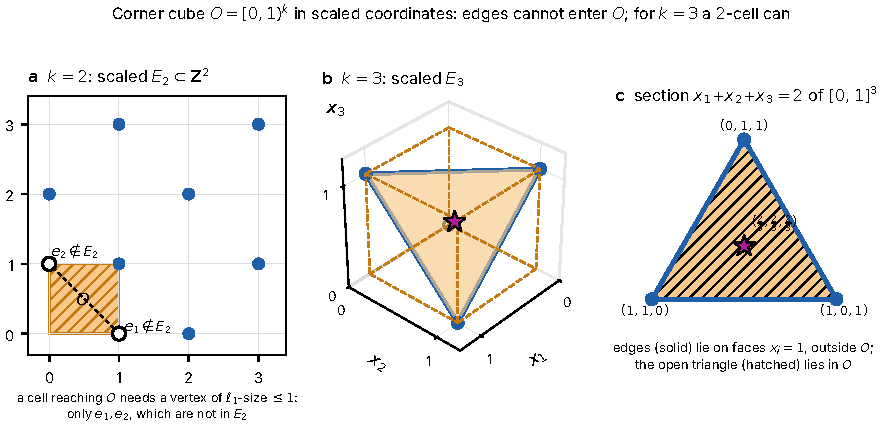
\includegraphics[width=0.98\textwidth]{fig05_dim2_vs_dim3}
\caption{Why dimensions two and three differ (\cref{thm:corner}(c)--(f), \cref{rem:dim}; scaled coordinates; \emph{theorem-level construction with exact coordinates}). (a)~$k=2$, scaled source $E_2\subset\Z^2$: a cell reaching the corner square $O=[0,1)^2$ would need a nonzero vertex of $\ell_1$-size $\le1$, i.e.\ $e_1$ or $e_2$, neither of which lies in $E_2$. (b)~$k=3$, scaled source $E_3\subset\Z^3$: the points $(1,1,0),(1,0,1),(0,1,1)$ of $\ell_1$-size $2$ \emph{do} lie in $E_3$; their triangle has its edges on faces $x_i=1$ of the unit cube, hence outside $O$, but its relative interior lies in $O$. The star is the centroid $(\frac23,\frac23,\frac23)$. (c)~The same triangle in the section $x_1+x_2+x_3=2$. The triangle is not a cell by itself; in \cref{fig:corner} it is part of the $2$-cell of $\Kabs(E_3,Q)$ that realises the obstruction.}\label{fig:dim}
\end{figure}

\subsection{The even-sum source}
\begin{theorem}[parametric obstruction for the even-sum family]\label{thm:evensum}
Let $k=3$, let $\Lambda'$ be rectangular and let the scaled source lattice be $E_3$ (index $2$), box $\tilde Q\ge(1,1,1)$. Then $U\not\subseteq U'$ iff $\max_i\tilde Q_i\ge2$. The smallest failing scaled box is $(1,1,2)$ up to permutation.
\end{theorem}
\prov{CW-0480}{P3-T3(h)}{PROVED}{FULL}
\begin{proof}
Both scalings by $\mathrm{diag}(o)^{-1}$ preserve the conformal order, Graver sets, cells, and the relation $U\subseteq U'$, so we work in scaled coordinates: $\Lambda=E_3$, $\Lambda'=\Z^3$, box $\tilde Q$. ($\Leftarrow$) Say $\tilde Q_3\ge2$. By \cref{prop:E25}, $g=(0,1,-1)$ and $h=(1,0,-1)$ are Graver vectors of $E_3$. The points $(0,0,2),(0,1,1),(1,0,1),(1,1,0)$ have even sum, are nonzero and lie in the box, so $\Pil((0,0,2);g,h)$ is a $2$-cell. Its point $(0,0,2)+\tfrac23g+\tfrac23h=(\tfrac23,\tfrac23,\tfrac23)$ lies in $O$, so $U\not\subseteq U'$ by \cref{thm:corner}(b). ($\Rightarrow$) If all $\tilde Q_i=1$, then $F=\{(1,1,0),(1,0,1),(0,1,1)\}$ ($(1,1,1)$ has odd sum): three points, so there is no $2$-cell; $U$ consists of points and edges, which miss $O$ by \cref{thm:corner}(d). \qedhere
\end{proof}
The cell and the point are drawn in \cref{fig:corner}. The first specimen of this phenomenon is the transition $13\to26$ of \cref{sec:threestage}, whose source cell $\Pil((0,0,2);(0,1,-1),(1,0,-1))$ is exactly this one.
\begin{figure}[tbp]\centering
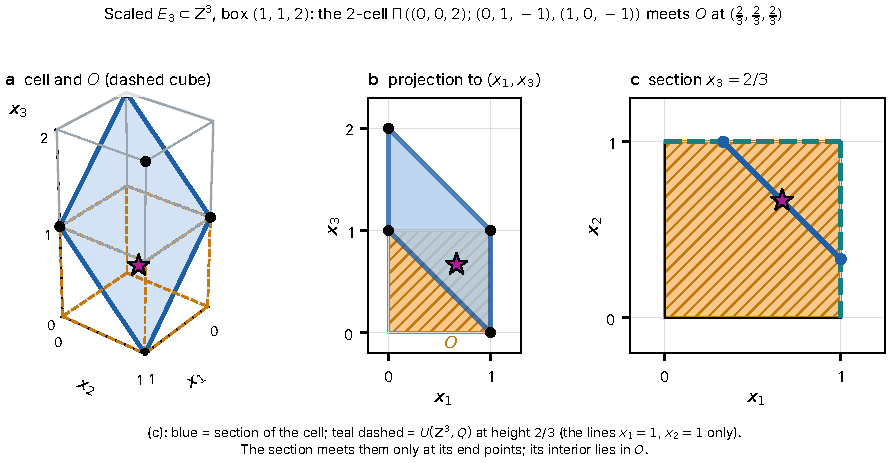
\includegraphics[width=0.98\textwidth]{fig06_corner_witness}
\caption{The exact corner-cube witness (\cref{thm:evensum}; scaled $\Lambda=E_3\subset\Lambda'=\Z^3$, box $(1,1,2)$; \emph{exact computation}). (a)~The $2$-cell $\Pil((0,0,2);(0,1,-1),(1,0,-1))$ of $\Kabs(E_3,Q)$ (a realised parallelogram), the five points of the fibre $F(E_3,Q)$ and the corner cube $O=[0,1)^3$ (dashed); the star is the witness $(\frac23,\frac23,\frac23)\in O$. (b)~Orthogonal projection to $(x_1,x_3)$, complementing the perspective view. (c)~The section $x_3=\frac23$: the section of the cell (blue segment from $(1,\frac13)$ to $(\frac13,1)$) has its interior in the open square $O$, while the target union $U(\Z^3,Q)$ at this height consists only of the lines $x_1=1$, $x_2=1$ (teal, dashed), met by the segment only at its end points. Hence the witness is not in $U(\Z^3,Q)$. All three panels show realised objects; none shows $\Kemb$.}\label{fig:corner}
\end{figure}

\subsection{The target union for \texorpdfstring{$b'=1$}{b\textquotesingle=1}}
\begin{corollary}[$U(\Z^k,Q)$]\label{cor:E27}
For $\Lambda'=\Z^k$ and $q\ge(1,\dots,1)$: $U(\Z^k,Q)=\{z\in Q:\max_iz_i\ge1\}$, a star-shaped (hence contractible) set. A convex polytope $\Pi\subseteq Q$ lies in it iff $\Pi\cap[0,1)^k=\emptyset$.
\end{corollary}
\prov{CW-0462}{E2-7}{PROVED}{ADAPTED}
\begin{proof}
\Cref{thm:corner}(a) with all $o_i=1$; star-shapedness about $q$: if $\max z_i\ge1$ then $\max(tz+(1-t)q)_i\ge1$ for $t\in[0,1]$ since $q_i\ge1$. \qedhere
\end{proof}
\begin{remark}[predictor]
For rectangular targets the criterion (b) can be evaluated cell by cell with one linear program per maximal source cell, never building the target complex. The release implements this; correctness is the content of (b). The procedure is an algorithm, not needed for the argument, and is not part of the theorem corpus of this manuscript (\texttt{CW-0481} is excluded for that reason).
\end{remark}
\prov{CW-0481}{P3-T4}{PROVED}{EXCLUDED}
